\chapter{序論}
 配管は、直管、曲管、バルブなど多様な部品で構成されており、建物の円滑な機能に不可欠な役割を担っている。
この配管システムは、パイプラインを通じて水、ガス、オイル、化学物質などの流体を輸送し、建物に必要なエネルギーを供給する重要な手段となっている。
また、配管システムを構築する際には、安全性や耐久性を含む条件を満たし、運用や保守が確実に行える設計が求められる[1][2]。\\
 近年、建物の安全性に対する意識が高まり、既存建物における配管モデルの再構築が重要視されている。
従来の配管モデルの構築方法では、作業者が配管の直径や長さを手作業で測定し、それをもとに図面を作成するのが一般的であった。
しかし、この方法には人的コストや時間的コストが高いという課題があり、過酷な環境下では作業者が危険にさらされる可能性があるといった問題も含まれている。
これらの課題を解決し、工事の迅速化を図るとともに、より高効率な配管モデルの構築方法が求められている。

\section{研究背景}
 Building Information Modeling(BIM)とは、建築物や土木構造物などの立体モデルをコンピュータ上で作成し、設計から維持管理までのプロセスをデジタル化する新しいワークフローである。
このBIMモデリングは従来の3Dモデリングとは大きく異なる特徴を持つ。
従来の3次元モデリングでは、平面図などの2次元図面を基に別途3次元モデルを作成していたため、図面と3次元モデルが連動せず、設計変更があるたびに両方を修正する必要があり、効率的ではなかった。
これに対して、BIMではデータが一元管理されており、一つのデータを修正するとすべての関連データが連動して自動的に修正される。
この仕組みにより、従来の方法よりも高い効率で作業を進めることが可能となる。\\
 また、配管の場合では、BIMモデルにおいてアイソメトリック(アイソメ)図と呼ばれる図面が重要な役割を果たしている。
アイソメ図は立体を斜めから見た視点で描画され、3つの座標軸(X, Y, Z)が互いに120度の間隔で配置される等角図である。
図\ref{fig:f1}にアイソメ図の例を示す。
\begin{figure}[htbt]
	\centering
	 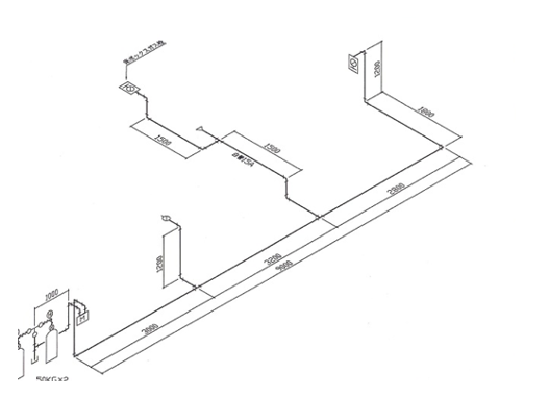
\includegraphics[height=80mm]{Figure/ex_iso.eps}
	 \caption{アイソメ図の例}
	 \label{fig:f1}
\end{figure}
設計図には平面図、立体図、系統図などさまざまな種類が存在するが、配管は複雑に交差することが多いため、左右や上下の視点だけでは正確に見分けることが難しい。
一方、アイソメ図は配管のルートや交差する配管の前後関係を立体的に表現するため、直感的に理解しやすく非常に有効な手法である。
従来のアイソメ図作成方法を図\ref{fig:f2}に示す。
\begin{figure}[htbt]
	\centering
	 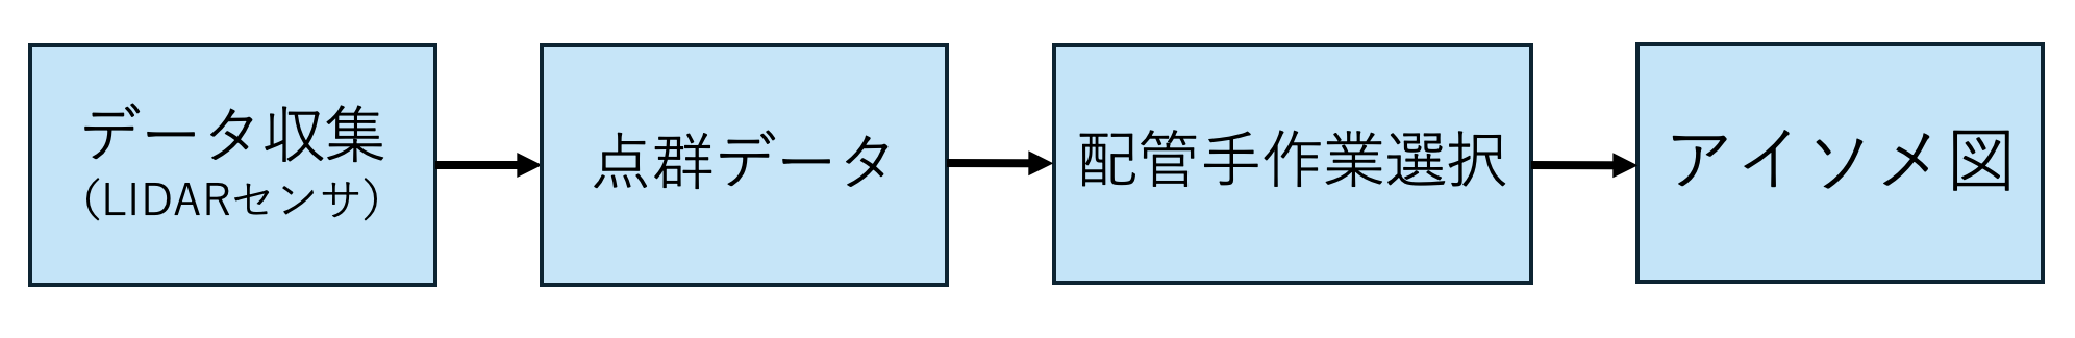
\includegraphics[height=22mm]{Figure/existing_research.eps}
	 \caption{従来のアイソメ図取得方法}
	 \label{fig:f2}
\end{figure}

 アイソメ図の取得にはLight Detection and Ranging(LIDAR)と呼ばれる、レーザー光を用いて離れた物体の形状や距離を測定できるセンサを使用していた。
LIDARセンサは、距離情報を活用して三次元情報を取得できるだけでなく、広い測定範囲や高い精度を持つ点が評価されている。
しかし、その一方で、他のセンサと比較して高価であるというデメリットがあり、多くの人々が容易に利用できるものではなかった。
また、点群データから人間が手作業で配管を検出する必要があるため、作業効率が低く、作業者の負担が大きいという問題もあった。\\

\section{既存研究}
 近年、機械学習を活用した物体認識技術の研究が広く行われており、急速な進展を遂げている。
機械学習とは、コンピュータが膨大なデータを基にパターンを学習し、そこから規則性を抽出する技術である。
その中でも特に深層学習は、人工知能の進化を支える中核的な技術として注目されており、人間の脳の構造を模倣したニューラルネットワークを用いた機械学習手法である。
従来の機械学習では、特徴量の設計を人間が行う必要があったが、深層学習では入力データから自動的に特徴量を抽出することが可能であり、これにより複雑な問題への対応が大きく進展した。
この技術は音声認識、点群データの解析、画像認識など、さまざまな分野で顕著な成果を挙げている。\\
 特に画像認識分野では、物体認識の自動化を深層学習によって実現することで、業務効率や生産性の向上に寄与するだけでなく、深刻化する人手不足の解消にも貢献することが期待されている。
近年の研究では、物体検出、セグメンテーション、さらに3次元位置および姿勢の推定といったタスクに注目が集まっており、それぞれの技術的概要や代表的な手法が活発に議論されている。
これらの技術的概要と代表的な手法を紹介する。\\
 まず、物体検出とは画像から物体を検出し、その位置とスケールを特定する技術である。
代表的な物体検出モデルの一つに、Region-Based Convolutional Neural Networks(R-CNN)が挙げられる。
R-CNNは主に二段階のアプローチを採用しており、まず画像中の物体候補領域を生成し、その後、その候補領域を分類器で検出するという手法である。
この手法では、物体候補領域の生成にSelective Searchアルゴリズムを使用し、各領域ごとに畳み込みニューラルネットワーク(CNN)を適用して物体を分類する。
この手法は高い精度を実現したものの、物体候補領域ごとに個別にCNNを適用する必要があり、計算コストが高く処理速度が遅いという課題が存在していた。
この課題を解決するため、Fast R-CNNやFaster R-CNNといった改良モデルが登場した。
Fast R-CNNでは、一度のCNN処理で画像全体の特徴マップを生成し、その特徴マップを物体候補領域ごとに利用することで計算効率を向上させた。
さらに、Faster R-CNNではRegion Proposal Network(RPN)と呼ばれるモジュールを導入し、物体候補領域の生成をニューラルネットワークで行うことで処理の効率化を図った。
これらの改良により、従来の手法と比較して高速かつ高精度な物体検出が可能となったが、リアルタイム処理には依然として限界があった。\\
 一方で、YOLO(You Only Look Once)という新しいアプローチが登場した。
このモデルの特徴は、従来の物体検出手法が二段階に分けて行っていた境界設定と物体検出の処理を、一度に行う点にある。
この「End-to-End」の手法により、推定速度が大幅に向上し、リアルタイムでの物体検出が可能となった。
YOLOの基本的な考え方は、画像をグリッドに分割し、各グリッドセルが物体を検出する責任を持つというものである。
具体的には、各セルが物体の存在を予測するとともに、その物体の境界ボックスの位置、スケール、そしてクラスラベルを同時に推定する。
このアプローチにより、物体候補領域の生成や個別の分類処理を省略し、一度の処理で物体の検出と分類を完了させることができる。\\
 続いて、セグメンテーションは、画像中のピクセル単位で物体を認識・分類する技術であり、物体検出をさらに詳細化した手法である。
セグメンテーションは大きく分けて、セマンティックセグメンテーション と インスタンスセグメンテーション に分類される。
セマンティックセグメンテーションにおいて代表的な手法として挙げられるのがDeepLabシリーズである。
DeepLabは、画像中のすべてのピクセルを特定のクラスに分類する技術として、その高い性能から広く使用されている。
このモデルの特徴は、空間的な解像度を維持しながら特徴抽出を行うために、「アトラス空間ピラミッドプーリング(ASPP)」を採用している点である。
ASPPは異なるスケールの情報を同時に取り込むことで、物体の大きさや位置に対するロバスト性を向上させる。
また、条件付きランダムフィールド(CRF)を活用することで、ピクセル単位での境界情報を精密に補正し、セグメンテーション結果の精度をさらに高めている。\\
 一方、インスタンスセグメンテーションにおける代表的なモデルとしてはMask R-CNNが挙げられる。
Mask R-CNNは、物体検出で広く用いられているFaster R-CNNを基盤に、各物体の領域(マスク)をピクセル単位で抽出する機能を追加したモデルである。
このモデルの大きな特徴は、物体検出の過程で領域ごとの特徴を抽出する際に「RoIAlign(Region of Interest Alignment)」という新しい手法を導入している点である。
RoIAlignは、従来の手法に比べて特徴マップからの領域情報抽出を高精度に行うことができ、マスク生成の精度を大幅に向上させた。
また、Mask R-CNNでは、物体の境界を滑らかに表現するためのマスクをピクセル単位で予測するため、従来のセグメンテーション手法に比べて高い精密さを誇る。\\
 次に、3次元位置姿勢推定について紹介する。
3次元位置姿勢推定は、物体の位置(X, Y, Z)に加えて、回転や向き(Roll, Pitch, Yaw)を推定する技術であり、6自由度の姿勢を推定可能である。
ここでは、この3次元位置姿勢推定タスクを「6D姿勢推定」と呼ぶことにする。
6D姿勢推定の手法としては、RGB画像のみを入力として使用する方法や、深度画像(Depth画像)を併用する方法が存在する。\\
 RGB画像のみを用いた代表的な手法の一つに、Generalizable Model-Free 6-DoF Object Pose Estimation from RGB Images(Gen6D)がある。
この手法の特徴は、一般的な6D姿勢推定モデルは物体の姿勢推定を行う際に対象物の3Dモデルを事前に作成し、それをデータセットに組み込む必要があった。
このプロセスは手間と時間を要し、運用効率を低下させる要因であったが、Gen6Dはこれらの課題を克服し、3Dモデルの準備を不要とする革新的なアプローチを提案している。
Gen6Dがこの課題を解決するために活用している技術の一つに、Structure from Motion(SfM)技術であるColmapがある。
Colmapは、異なる視点から撮影された複数の2D画像(参照画像)をもとに3D点群データを再構築する技術であり、これにより3Dモデルを用意することなく、物体の6D姿勢を推定できる仕組みを提供している\\
 Gen6Dは、物体の姿勢推定を行うために、物体検出(Detector)、画像マッチング(Selector)、姿勢補正(Refiner)の3つのステップを経る。
物体検出では参照画像をもとに物体の領域を検出し、画像マッチングでは得られた領域画像と最も近い視点を持つ参照画像を選択する。
この参照画像はColmapを活用することで内部パラメータや外部パラメータを取得することが可能となり、その視点情報を用いて物体の初期姿勢を推定することができる。
また、初期姿勢には誤差が生じる可能性があるため、選択された参照画像からさらに複数枚の画像を使用し、姿勢を補正することで最終的な姿勢推定の精度を向上させる。\\
 しかし、Gen6Dにはいくつかの課題が存在する。
特に、推論時には3Dモデルを使用する必要はないが、学習時にSfMを用いて3D点群データを再構築する必要があるため時間と労力がかかる。
また、対象物体が前の物体によって隠れてしまうようなオクルージョンと呼ばれる状況では、正確な姿勢推定が困難になるという問題があった。\\
 一方、RGB-D画像を使用した手法として、Segment Anything Model for 6D Pose Estimation(SAM-6D)が挙げられる。
SAM-6Dは、Segment Anything、Object Matching、Coarse Point Matching、Fine Point Matchingの4つのステップを通じて物体の6D姿勢を推定する手法である。
最初のステップであるSegment Anythingでは、SAMを用いて入力画像内の対象物体になり得る物体を全てセグメント化する。
SAMは、ポイントやボックス、マスクなどの多様なプロンプトに基づいて有効なマスクを生成できるモデルであり、これによりゼロショットで多くのセグメント提案が生成される。
Object Matchingでは、ターゲットオブジェクトとの一致度が、セマンティクス、外見、形状といった複数の要素に基づいて評価される。
具体的には、事前に用意されたテンプレート画像を使って、セグメント提案がターゲットオブジェクトとどの程度一致するかをスコアリングする。
続いて、Coarse Point Matchingでは、ターゲットオブジェクトの3Dモデルからレンダリングされたテンプレート画像を基に、画像マッチングを行う。
この過程で、物体の初期的な姿勢が推定される。
最後のステップであるFine Point Matchingでは、入力されたDepth画像から点群データを取得し、それを使用してオブジェクトの3Dモデルの点群と対応付けを行う。
これら4つのステップが連携することで、精密な6D姿勢推定を実現している。\\
 また、このSAM-6Dモデルは、オクルージョンによる影響を軽減するために、バックグラウンドトークンという仮想点を導入している。
この仮想点はDepth画像を利用できることに起因しており、欠損領域が存在する場合においても、物体の3Dモデルとの対応付けを行うことが可能となる。
このアプローチは、Gen6Dで課題となっていたオクルージョン問題に対応する新たな手法として注目されている。


\section{研究目的}
本研究では、従来のアイソメ図取得方法における課題を解決するために新たな手法を提案し、その有効性を検証することを目的とする。
図\ref{fig:f3}に新規のアイソメ図取得方法を示す。\\
\begin{figure}[htbt]
	\centering
	 \includegraphics[height=33mm]{Figure/new_research.eps}
	 \caption{新規のアイソメ図取得方法}
	 \label{fig:f3}
\end{figure}

提案手法には以下の2つの主な特徴がある。
1つ目は、従来のLIDARセンサに代わりRGB-Dカメラを使用する点である。
RGB-DカメラはLIDARセンサに比べて低コストでありながら、Depth画像を活用することで三次元情報を取得することが可能である。
この変更により、一般的に使用可能なアプリケーションとして提供することが実現できる。
2つ目は、従来は人間による手作業に依存していた配管検出処理を深層学習によって自動化し、効率を大幅に向上させる点である。
特に、6D姿勢推定を活用することで配管の向きや位置を正確に特定し、配管間の接続関係を把握することが可能となる。
この手法により、配管の接続情報を正確に推論し、最終的にはアイソメ図作成に必要なCADデータへの変換が実現できる。\\
 本研究の主な貢献は以下の通りである。
1つ目は、RGB-Dカメラを利用した低コストで汎用性の高いアイソメ図作成方法を提案し、広く使用可能なアプリケーションを提示したことである。
2つ目は、大規模配管設備のアイソメ図生成を実現するために、仮想環境で配管を構築し、実環境との差異を最小限に抑えた状態でアイソメ図を生成できるようにした点である。
3つ目は、アイソメ図作成に必要な6D姿勢推定モデルを比較検証し、本研究に適したモデルを選定したことである。


\section{本論文の構成}
本論文の構成は以下のようになる.
第1章では研究背景、既存研究、研究目的について述べる。
研究背景では、Building Information Modeling (BIM) の概要や、従来のアイソメ図取得方法について詳述する。
既存研究では、深層学習を用いた画像認識分野に関する研究を紹介し、これまでの手法との違いを明確にする。
研究目的では、本研究で提案する新たな手法とその貢献について述べる。

第2章では、深層学習を用いた配管6D姿勢推定およびアイソメ図作成に至る方法とその流れについて説明する。
第2.1節では本章の全体構成を紹介し、全体的な流れを把握できるようにする。
第2.2節では、RGB-D画像に基づく配管6D姿勢推定の方法について述べ、実際に使用する物体検出やセグメンテーション、6D姿勢推定モデルについて説明する。
第2.3節では、得られた6D姿勢推定情報を基にアイソメ図を作成する手法について述べる。
具体的には、配管の接続関係を推論し、アイソメ図を作成するためにCADデータに変換する方法を説明する。

第3章では、実環境における配管設備を用いた検証実験を通じて、提案手法の有効性を検証する。
第3.1節では使用する機材について説明し、必要な技術的要素を紹介する。
第3.2節では、データセットの収集方法およびデータセットの作成方法について説明する。
第3.3節では、提案手法の評価指標について述べ、実験結果の比較基準を明確にする。
第3.4節では、提案手法の有効性を確認するために行った実験結果について報告する。

第4章では、仮想環境における大規模配管設備での検証実験の結果を示す。
第4.1節では仮想環境の構築方法について説明し、仮想環境と実環境との差異を最小化するために導入したセンサーモデルについても詳述する。
第4.2節では、仮想環境で取得した配管画像を用いてアイソメ図を生成した結果を示し、その精度や効率について議論する。

第5章は結論にあたり、本研究の成果を総括し、今後の課題と展望について述べる。
